\documentclass[11pt,]{article}
\usepackage{lmodern}
\usepackage{amssymb,amsmath}
\usepackage{ifxetex,ifluatex}
\usepackage{fixltx2e} % provides \textsubscript
\ifnum 0\ifxetex 1\fi\ifluatex 1\fi=0 % if pdftex
  \usepackage[T1]{fontenc}
  \usepackage[utf8]{inputenc}
\else % if luatex or xelatex
  \ifxetex
    \usepackage{mathspec}
    \usepackage{xltxtra,xunicode}
  \else
    \usepackage{fontspec}
  \fi
  \defaultfontfeatures{Mapping=tex-text,Scale=MatchLowercase}
  \newcommand{\euro}{€}
    \setmainfont{Georgia}
\fi
% use upquote if available, for straight quotes in verbatim environments
\IfFileExists{upquote.sty}{\usepackage{upquote}}{}
% use microtype if available
\IfFileExists{microtype.sty}{%
\usepackage{microtype}
\UseMicrotypeSet[protrusion]{basicmath} % disable protrusion for tt fonts
}{}
\usepackage[margin=0.5in]{geometry}
\usepackage{graphicx}
\makeatletter
\def\maxwidth{\ifdim\Gin@nat@width>\linewidth\linewidth\else\Gin@nat@width\fi}
\def\maxheight{\ifdim\Gin@nat@height>\textheight\textheight\else\Gin@nat@height\fi}
\makeatother
% Scale images if necessary, so that they will not overflow the page
% margins by default, and it is still possible to overwrite the defaults
% using explicit options in \includegraphics[width, height, ...]{}
\setkeys{Gin}{width=\maxwidth,height=\maxheight,keepaspectratio}
\ifxetex
  \usepackage[setpagesize=false, % page size defined by xetex
              unicode=false, % unicode breaks when used with xetex
              xetex]{hyperref}
\else
  \usepackage[unicode=true]{hyperref}
\fi
\hypersetup{breaklinks=true,
            bookmarks=true,
            pdfauthor={},
            pdftitle={},
            colorlinks=true,
            citecolor=blue,
            urlcolor=blue,
            linkcolor=magenta,
            pdfborder={0 0 0}}
\urlstyle{same}  % don't use monospace font for urls
\setlength{\parindent}{0pt}
\setlength{\parskip}{6pt plus 2pt minus 1pt}
\setlength{\emergencystretch}{3em}  % prevent overfull lines
\setcounter{secnumdepth}{0}

%%% Use protect on footnotes to avoid problems with footnotes in titles
\let\rmarkdownfootnote\footnote%
\def\footnote{\protect\rmarkdownfootnote}

%%% Change title format to be more compact
\usepackage{titling}

% Create subtitle command for use in maketitle
\newcommand{\subtitle}[1]{
  \posttitle{
    \begin{center}\large#1\end{center}
    }
}

\setlength{\droptitle}{-2em}
  \title{}
  \pretitle{\vspace{\droptitle}}
  \posttitle{}
  \author{}
  \preauthor{}\postauthor{}
  \date{}
  \predate{}\postdate{}

\usepackage{booktabs}


\begin{document}

\maketitle


\section{Specific Aims}\label{specific-aims}

Medical research significantly benefits from the development and
proliferation of imaging-related analysis packages, particularly those
softwares which have been tailored for specific application domains.
Although several such established packages exist for \emph{neuroimaging}
research (e.g., FSL, FreeSurfer, AFNI, SPM), no such package exists for
pulmonary imaging analysis. The primary goal of this proposal is to
develop a robust, open-source image analysis toolkit and dissemination
platform, along with annotated data, specifically targeted at the
pulmonary research community.

Although methodological research is continually being presented at
conferences and published in various venues, the unfortunate reality is
that much of this work exists strictly in ``advertisement'' form.
Oftentimes the underlying code is unavailable to other researchers or is
implemented in a limited manner (i.e., strictly as proof-of-concept
software). Frequently, crucial parameter choices are omitted in the
corresponding publication(s) which makes external implementations
difficult. In addition, the data used to showcase the proposed
methodologies are often private and actual data visualization is limited
to carefully selected snapshots for publication (i.e., advertisement)
purposes which might not be representative of algorithmic performance.
Finally, many of these analysis methods are patented and/or integrated
into proprietary commercial software packages which severely limits
accessibility to researchers.

As a corrective alternative, this proposal will provide an open-source
software toolkit for core pulmonary image analysis tasks across multiple
modalities, many of which we have proposed previously in past
publications. These basic tasks include pulmonary image registration,
template building for cross-sectional and longitudinal (i.e.,
respiratory cycle) analyses, and functional and structural lung image
segmentation. In addition to the software, we will provide both the
input and output data consistent with open-science principles not only
so that other users can it to reproduce our results, but it will also
allow researchers to use it in an unrestricted manner in their own
studies. Formally, this proposal is defined by the following specific
aims:

\begin{itemize}
\itemsep1pt\parskip0pt\parsep0pt
\item
  \textbf{Specific Aim 1:} \textbf{Develop a set of open-source software
  tools for CT, proton, and He-3 pulmonary computational analysis.}
  These open-source software tools will specifically target pulmonary
  image analysis and comprise core application functions such as
  inspiratory/expiratory registration for inferring pulmonary
  kinematics, ventilation-based segmentation, lung and lobe estimation,
  airway segmentation, and calculation of clinical indices for
  characterization of lung development and pathology.
\item
  \textbf{Specific Aim 2:} \textbf{Provide multiple sets of multi-modal
  annotated lung data (CT, proton, and He3) for unrestricted public
  use.} In addition to the public unavailability of the algorithms used
  to produce the results discussed in certain publications, the input
  and output data is also typically not available. Such availability
  would be invaluable to other researchers in the community for
  appropriation for their own purposes including algorithmic performance
  assessment and running the proposed prior-based methods requiring
  annotated input data.
\item
  \textbf{Specific Aim 3:} \textbf{Evaluate and disseminate multiple
  complete studies with input data from multiple investigators to
  showcase the utility of the tools and data provided with this
  proposal.} In order to maximize the utility of the proposed pulmonary
  image analysis framework, our proposal also includes making available
  the input data from multiple researchers (with their permission)
  involved in a variety of pulmonary research questions and the output
  data produced by the framework. Among other purposes, this
  contribution will provide complete, concrete examples demonstrating
  usage of the proposed contribution.
\end{itemize}

As principal developers of the popular, open-source ANTs (Advanced
Normalization Tools) package, we have extensive experience in the
development of well-written software that has gained much traction in
the neuroscience community. We have also participated in several image
analysis competitions for a variety of applications (neuro, pulmonary,
and cardiac) and data scaling and believe that this will also contribute
to our success in accomplishing the goals of this application.

\newpage

\section{Research Strategy}\label{research-strategy}

\subsection{\textbf{3(a) Significance}}\label{a-significance}

Well-vetted and publicly available software is a significant benefit to
targeted research communities. For example, the neuroscience community
has greatly benefited from highly evolved software packages such as
FreeSurfer {[}1{]}, the FMRIB Software Library (FSL) {[}2{]}, the
Analysis of Functional NeuroImages (AFNI) package {[}3{]}, and the
Statistical Parametric Mapping (SPM) package {[}4{]}. Performing a
pubmed query for any one of these softwares every year for the past
decade (cf Figure 1) illustrates the growing use of such packages and
the research studies that are produced as a result. However, despite the
absolute number of articles produced using such software and the
year-by-year usage increase, no such analogous set of tools exist for
pulmonary-specific research. In fact, in a recent review of CT- and
MRI-derived biomarkers for pulmonary clinical investigation, the
authorial consensus is that ``universally available image analysis
software'' is a major hinderance to more widespread usage of such
imaging biomarkers {[}5{]}.

\begin{figure}[htbp]
\centering
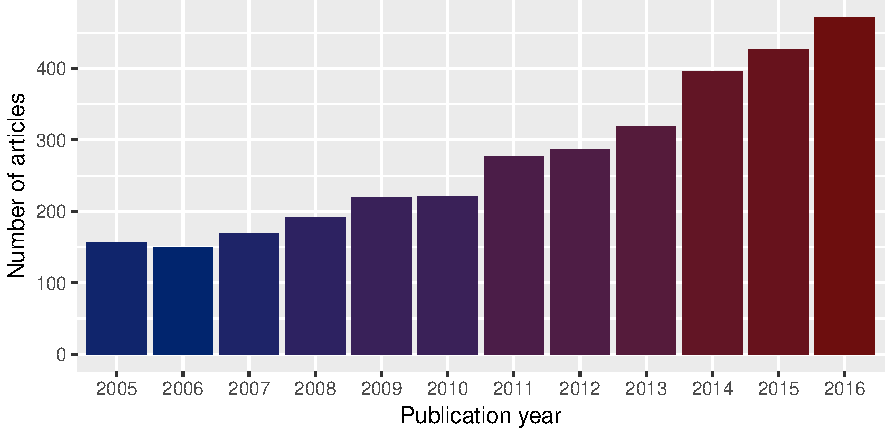
\includegraphics{stitched_files/figure-latex/pubmedQuery-1.pdf}
\caption{Number of articles per year which use common, publicly
available neuroimaging analysis packages (i.e., FreeSurfer, AFNI, FSL,
and SPM). Although the benefits seem clear for the neuroscience
community, analogous efforts within the pulmonary community have yet to
be undertaken.}
\end{figure}

Medical image analysis libraries (e.g., the NIH-sponsored Insight
ToolKit) provide extensive algorithmic capabilities for a range of
generic image processing tasks. However, tailored software packages for
certain application domains (e.g., lung image analysis) are not
available despite the vast number of algorithms that have been proposed
in the literature. Similar deficiency within the neuroscience community
has been one of the primary motivations for the inception and continued
development of our Advanced Normalization Tools (ANTs). ANTs takes
advantage of the mature Insight ToolKit in providing an optimal software
framework for building scripts and programs specifically for
neuroimaging. For example, the following core neuroimage processing
algorithms have been made available through our ANTs toolkit (complete
with examples and developer-tuned parameters) and have been used
extensively by our group and others:

\begin{itemize}
\itemsep1pt\parskip0pt\parsep0pt
\item
  brain normalization {[}6, 7{]},
\item
  brain template generation {[}8{]},
\item
  skull-stripping or brain extraction {[}9, 10{]},
\item
  prior-based Bayesian brain tissue segmentation {[}6{]},
\item
  cortical gray matter thickness estimation {[}10, 11{]},
\item
  brain tumor segmentation {[}12{]}, and
\item
  cortical labeling {[}13, 14{]}.
\end{itemize}

In addition to public availability, some of these algorithms have been
showcased in international competitions and have performed extremely
well {[}15, 16{]}.

Analogously, several algorithmic categories exist for lung image
analysis which, as we have stated previously, do not exist in any
comprehensive, publicly available package. An extensive survey
concentrating on the years 1999--2004 is given in {[}17{]} which covers
computer aided diagnosis of lung disease and lung cancer in CT (i.e.,
detection and tracking of pulmonary nodules) and provides an overview of
the many relevant segmentation methods for pulmonary structures.
Although many algorithms existed at the time, continued technical
development has only increased the number of available algorithms.
Following is a small sampling of more recently reported techniques for
CT analysis:

\begin{itemize}
\itemsep1pt\parskip0pt\parsep0pt
\item
  whole lung differentiation from the chest wall (e.g., {[}18--21{]})
\item
  bronchial structure extraction (e.g.,{[}22, 23{]}; the many
  submissions to the recent Extraction of Airways from CT (ExACT)
  challenge of the 2nd International Workshop on Pulmonary Image
  Analysis {[}24{]}),
\item
  vasculature segmentation (e.g., {[}25, 26{]}),
\item
  lobe and/or fissure detection (e.g., {[}27, 28{]}), and
\item
  feature extraction and classification (e.g., {[}29--31{]}).
\end{itemize}

Since this list is restricted to CT image analysis, inclusion of
additional techniques specific to other modalities will have additional
benefit. For example, ventilation-based segmentation for analysis of
ventilation lung imaging {[}32{]} will also have significant impact in a
comprehensive lung image analysis suite.

Important in any methodological discussion is the crucial importance of
parameter selection which requires domain-specific experience. For
example, although ANTs performance in brain registration has been
independently evaluated and found to be of relatively high quality
{[}Klein2009{]}, tailoring our registration tool in the EMPIRE10
challenge (Evaluation of Methods for Pulmonary Image REgistration 2010)
required significant empirically-based tuning. In addition, new
innovations in diffeomorphic registration technology has led to a
Symmetric Normalization B-spline variant which has demonstrated
preferred normalizations {[}33{]}, particularly for pulmonary data
{[}34{]}. Note that the goals of this proposal would significantly
support the National Library of Medicine's own open-source directives in
that all software would be developed using the established Insight
ToolKit's coding and testing standards with the eventual idea that much
(if not all) of the actual code would be contributed for inclusion in
future versions of the Insight ToolKit.

It should also be noted that open-source software, in general, has
documented benefits within the targeted communities for which it is
developed and supported. In addition to the increase in research output
illustrated earlier, open-source permits students and researchers to
learn specific computational techniques in a social environment
{[}35{]}. This, in turn, provides motivation for user-based support
including potential contributions such as bug fixes and feature
additions. Additional analyses have shown the tremendous cost savings
that open-source software yields {[}36{]}.

\subsection{\textbf{3(b) Innovation}}\label{b-innovation}

Given the lack of open-source solutions for pulmonary image analysis,
the proposal goals would produce an innovative framework for
corresponding research. Many algorithms have been proposed in various
technical venues but that which we propose would provide well-vetted and
easy-to-use implementations of specific robust methodologies, many of
which have been developed by our group.

An additional innovative component we are proposing is the inclusion of
data and detailed instructions for generating reproducible,
multimodality pulmonary studies using the proposed package with input
data from several of our external collaborators and colleagues.
Specifically, we have asked several scientists and researchers who are
familiar with our work to provide imaging data of various modalities
which we will then process using the proposed toolkit. These processed
data will then not only be returned to the corresponding providers with
detailed instructions on how to obtain these results in their own labs
but will also be provided to the public for any interested researcher to
reproduce the results. Given the different image acquisition sources,
this strategy should also demonstrate the robustness of our tools.

Included in these analyses will be studies dealing with our own data.
Clinical findings will be published in traditional venues (e.g., Chest)
for the interested researcher. In addition, we will provide all image
data and the quantitative analysis scripts as a companion release to
accompany the paper (e.g., see previous similar offerings from our group
{[}10, 33{]}). Such a comprehensive clinical investigation using these
tools will not only provide insight into the specifics of certain
pulmonary pathologies but will also provide a tangible mechanism for
using the tools created with this proposal.

\subsection{\textbf{3(c) Approach}}\label{c-approach}

\textbf{Specific Aim 1.} To develop a set of open-source software tools
for CT, proton, and He-3 pulmonary computational analysis. Development
will include several basic tools:

\emph{B-spline-based Symmetric Normalization.} A thorough comparative
evaluation with the well-known ANTs SyN algorithm was performed with a
B-spline variant. The evaluation utilized multiple publicly available,
annotated brain data sets and demonstrated statistically significant
improvement in label overlap measures {[}33{]}. We also used the
EMPIRE10 challenge framework to provide an additional comparison in the
context of pulmonary CT image registration {[}37{]}. Due to the
performance of this new variant, it has become the preferred
transformation model for small deformation image registration problems
(e.g., lung and cardiac {[}38{]} applications).

\emph{Multi-feature CT and multi-modal MRI template generation.} we
generate subject-specific templates directly from the image data. Given
the variability in lung shape across populations and the lack of
publicly available lung atlases, generating population- or
subject-specific templates enhances the accuracy of the longitudinal
analysis described in this work. Applicable to pulmonary data is the
template construction algorithm described in {[}8{]} which was applied
to T1-weighted brain data. However, the simultaneous acquisition of the
3He and 1H images lends itself to multimodal processing {[}12{]} in
which both modalities are used to simultaneously produce 3He and 1H
templates. This process is represented in Fig. 1 for a single subject.

\emph{Atlas-based lung segmentation.} Identification of anatomical
structure in MRI is often a crucial preprocessing step for
quantification of morphological features or functional information.
Quantitative regional analysis often requires the identification of lung
and lobar anatomy. Although much algorithmic research for lung
segmentation has been reported in the CT literature {[}39{]}, co-opting
such technologies is complicated by MRI-specific issues such as RF coil
inhomogeneity, presence and resolution of structural detail, and the
absence of a physically-based intensity scaling.

We recently proposed a multi-atlas approach for automatically segmenting
the left and right lungs in proton MRI {[}34{]}. Multi-atlas approaches
to segmentation have proven highly successful in neuroimaging
{[}Reference 13;Wang:2013aa{]} which translates readily to a pulmonary
context. Many current strategies for lung image segmentation employ
low-level processing techniques based on encodable heuristics.
Consensus-based strategies, in contrast, optimize the prior knowledge
applied to a specific segmentation problem (cf Figure 2).

\begin{figure}[htbp]
\centering
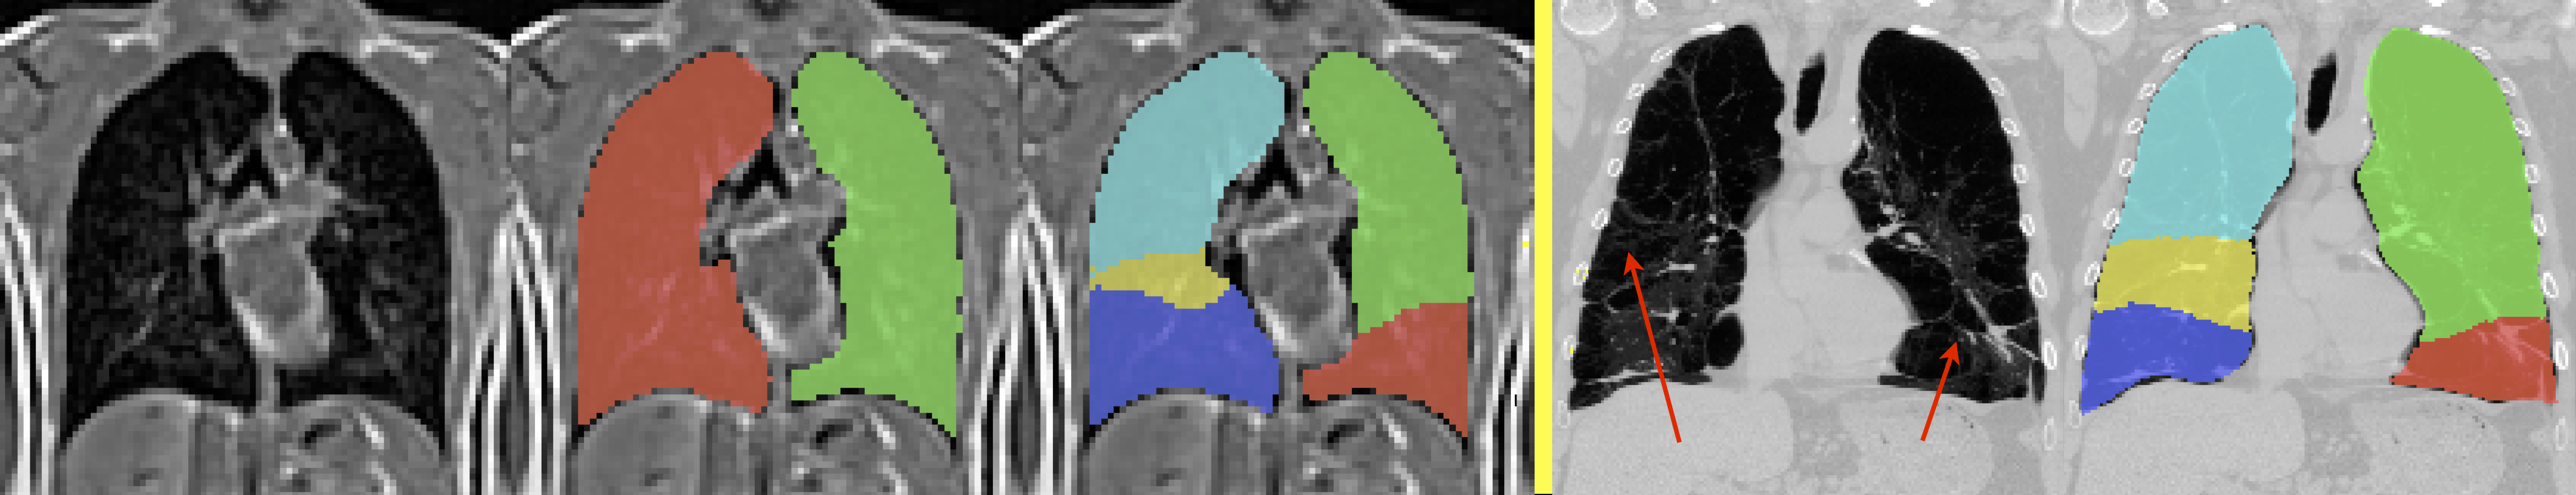
\includegraphics{Figs/lungEstimation.png}
\caption{Sample lung and lobe estimation results in both proton MRI and
CT using our atlas-based strategy. (Left) Lung segmentation and lobe
estimation results for the given proton MRI. Although lobe estimation is
dependent solely on the warped atlases, we are able to obtain accurate
estimates of lobes which are useful for more regional analysis and
provide a more intuitive and universal subdivision of the lungs than
previous partitioning schemes. (Right) The utility of this method
extends to CT where the integrity of lobar anatomical markers (such as
the lack fissures illustrated by the red arrows) have been compromised
due to disease.}
\end{figure}

\emph{Atlas-based lobe estimation.} For regional investigation of
certain lung pathologies and conditions, it is often useful to quantify
measurements of interest within more localized regions, such as the
lobes. However, as mentioned previously, there is little (if any) usable
information in proton MRI for image-based lobar segmentation which has
led to alternative geometric subdivisions which are ad hoc,
non-anatomical, and do not adequately address intra- and inter-subject
correspondences. However, we can take advantage of inter-subject
similarities in lobar geometry to provide a prior-based estimation of
lobar divisions using a consensus labeling approach (cf Figure 2).

To generate the lobe segmentation in a target proton lung image, we
first generate the binary lung mask for the proton lung image as
described in the previous subsection. We then register the set of CT
lung masks to the target binary lung mask using the same registration
approach mentioned earlier {[}33{]}. Subsequently, we warp the set of CT
lobe labels to the target image using the CT mask-to-proton mask
transformation. Since we have no intensity information inside the target
lung mask and CT atlas lung masks, we use a simply majority voting
strategy to generate the optimal labeling for the target image.
Following the majority voting, we remove any labelings outside the lung
mask and assign any unlabeled voxels with the label closest in distance
to that voxel.

\emph{Ventilation-based image segmentation.} Developments in MRI
research utilizing noble gases, such as 3He and 129Xe, have demonstrated
the capability of visualizing alveolar and bronchial air spaces.
Currently, hyperpolarized 3He MRI is a low-risk investigatory technique
that provides high spatial and temporal resolution images of the air
spaces of the lungs and has been used to investigate a variety of lung
diseases. Automated or semiautomated approaches for classifying areas of
varying degrees of ventilation are of potential benefit for facilitating
such investigation.

In {[}32{]}, we presented an automated algorithmic pipeline for
ventilation-based partitioning of the lungs in hyperpolarized 3He and
129Xe MRI. Since then, we have continued to improve this segmentation
pipeline including the recent introduction of an ANTs-based
implementation of the patch-based denoising protocol described in
{[}40{]}. An example of a set of longitudinal segmentation results are
provided in Figure 3.

\begin{figure}[htbp]
\centering
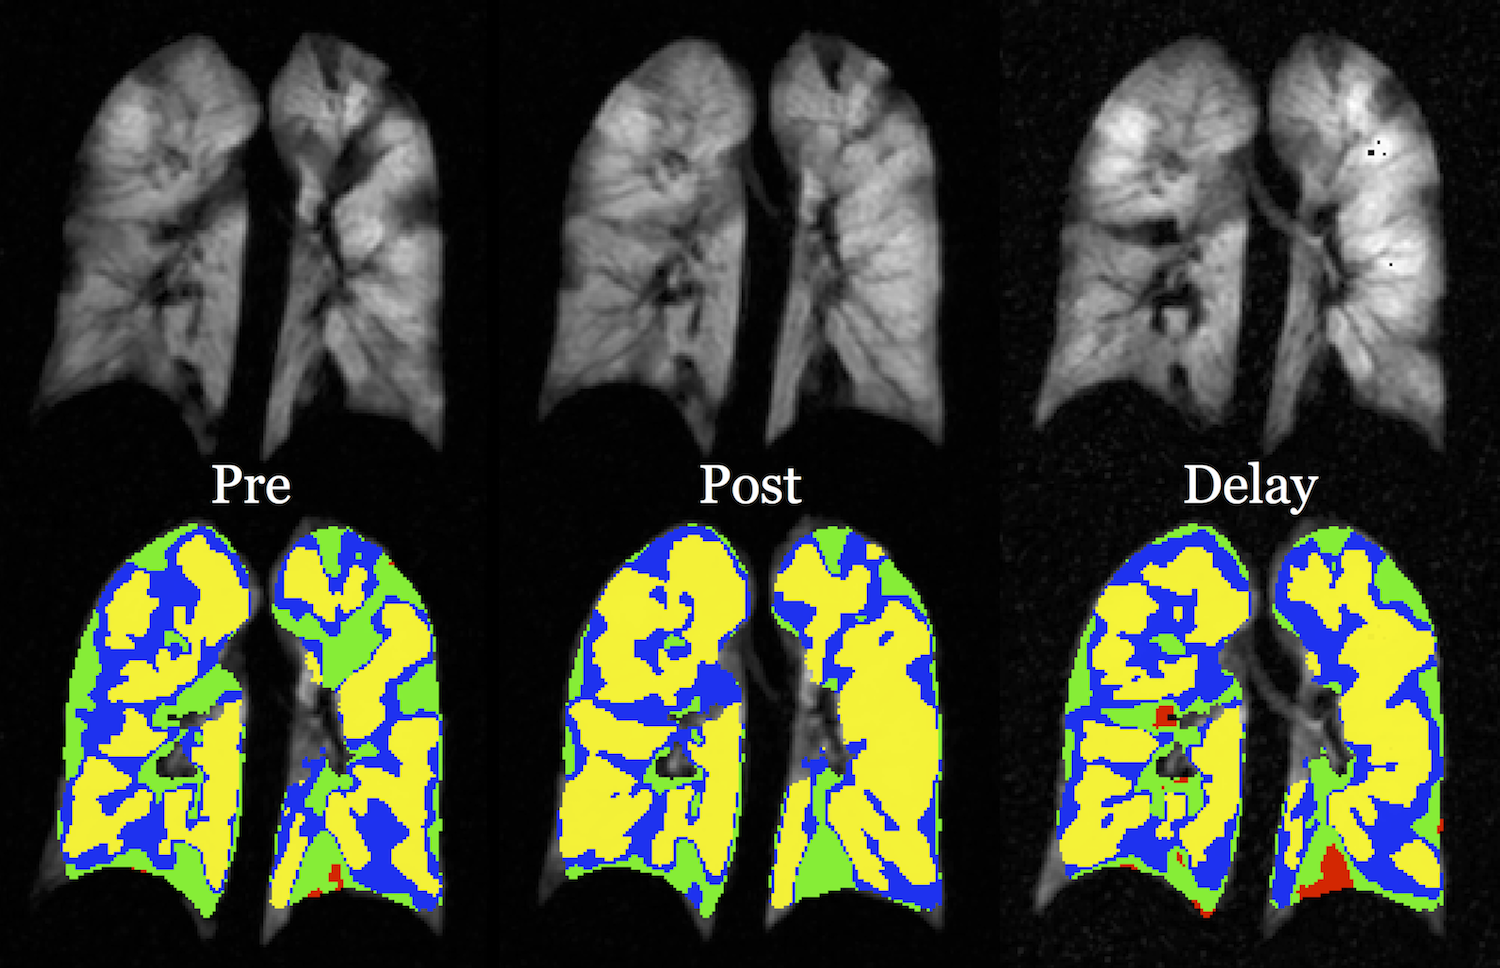
\includegraphics{Figs/prePostAlbuterol.png}
\caption{Pulmonary functional segmentation using the algorithmic
framework first described in {[}32{]} for hyperpolarized 3He MRI. These
data were taken from a current study looking at the implications in
ventilation pre- and post-albuterol intake including an additional
acquisition at some delay period following the post-albuterol imaging.
The ventilation-based segmentation is as follows: red = no ventilation,
green = poor ventilation, blue = normal ventilation, and yellow = normal
to hyper-ventilation. Note the improvement in both the qualitative
assessment of the ventilation map (top) and the corresponding
segmentation time course (bottom) followed by an approximate return to
pre-albuterol conditions following the delay period.}
\end{figure}

\emph{Quantitative CT indices.} Imaging biomarkers for characterizing
emphysema in CT have have been well researched, although there are ample
opportunities to refine these methods as well as to introduce more
advanced approaches. Examples of the latter include texture analysis for
identifying the centrilobular and groundglass opacities and fractal and
connectivity approaches to differentiate centrilobular from panlobular
emphysema. The indices for CT image analysis can roughly be divided into
those that characterize the pulmonary parenchyma and those that
characterize the airways. The former are important for subjects with an
emphysematous component of disease, whereas the latter are important for
subjects with a bronchitic component of disease. Such indices can also
be studied not only at any particular single time point, but also for
changes with time. The addition of quantitative morphologic measurements
of the airways provides an assessment of the contribution of airway
changes to chronic lung disease.

Table 1 provides an historical overview of the type of discriminative
measurements that have been used for CT lung assessment. \emph{An
important premise of this proposal is that many of these measurements
can also be directly applied to discriminative analysis using 3HeMRI for
a variety of lung diseases.} We have already implemented many of these
image features and have contributed the result of our work to the
Insight Toolkit (ITK) of the National Institutes of Health (e.g., {[}41,
42{]}). As an open-source repository for medical image analysis
algorithms, contribution of our work to the ITK allows researchers full
access to the latest image analysis algorithms in addition to avoiding
research redundancy. It is also beneficial in that the entire ITK
community participates in the vetting of the software library.

{[}7;9;16;18;19;24;25;26;30;31;32;33;37;41;46;54;55;56;57;59;61;63;64;65;66;68;70;74;76;77;82;83;84;85;92;98;110;111;112;114;117;118;120;121{]}

\emph{Airway and vessel segmentation.} We should propose to implement
something here. We should look at the Slicer/VMTK airway segmentation
model.

\textbf{Specific Aim 2.} To provide multiple sets of multi-modal
annotated lung data (CT, proton, and He3) for public use.


\begin{table}[!t]
  \small
  \begin{minipage}{0.33 \linewidth}
   \vspace{2mm}
   \centering
    \begin{tabular}[t]{c}
    {\bf Volumetric Tissue Indices}  \\
    \cmidrule[1pt](lr){1-1}
    lung volume   \\
    lobar volume  \\
    surface area  \\
    surface area to volume ratio  \\
    total lung weight  \\
    tissue/airspace volumes of lung \\
    inspiration vs. expiration$^*$ \\
    \\
    {\bf Airway Indices} \\
    \cmidrule[1pt](lr){1-1}
    airway luminal diameter and area  \\
    airway wall thickness  \\
    percentage wall area   \\
    thickness to diameter ratio  \\
    airway branch angles  \\
    airway segment length  \\
    airway wall volumes (segmental and total)$^*$ \\
    inspiration vs. expiration  \\
    \\
    {\bf Distribution of LAA Heterogeneity}  \\
    \cmidrule[1pt](lr){1-1}
    10 partitions (std of $15^{th} \%$)  \\
    slopes of density mask curves  \\
    $\%$ size distribution of LAA areas \\
    volumetric cluster analysis \\
    inner core vs. outer rind \\
    inspiration vs. expiration$^*$ \\
    \\
   \end{tabular}
   \end{minipage}
  \hspace{0cm}
  \begin{minipage}{0.33 \linewidth}
   \vspace{-8mm}
    \centering
    \begin{tabular}[t]{c}
    {\bf Cooccurrence Matrix Texture Indices}  \\
    \cmidrule[1pt](lr){1-1}
    energy  \\
    inertia  \\
    contrast  \\
    entropy  \\
    correlation  \\
    inverse difference moment \\
    cluster shade$^*$ \\
    cluster prominence$^*$ \\
    Haralick's correlation$^*$ \\
    \\
    {\bf Run-length Matrix Texture Indices}  {} \\
    \cmidrule[1pt](lr){1-1}
    short run emphasis  \\
    long run emphasis   \\
    grey level non-uniformity   \\
    run-length non-uniformity  \\
    run percentage  \\
    low grey level run emphasis$^*$ \\
    high grey level run emphasis$^*$ \\
    short run low grey level emphasis$^*$ \\
    short high grey level run emphasis$^*$ \\
    long run low grey level emphasis$^*$ \\
    long high grey level run emphasis$^*$ \\
    inspiration vs. expiration$^*$\\
    \\
    \end{tabular}
   \end{minipage}
  \hspace{0cm}
  \begin{minipage}{0.33 \linewidth}
   \vspace{0mm}
    \centering
    \begin{tabular}[t]{c}
    {\bf Attenuation Histogram Statistics}  \\
    \cmidrule[1pt](lr){1-1}
    attenuation mean  \\
    attenuation variance  \\
    attenuation skewness  \\
    attenuation kurtosis  \\
    attenuation grey level entropy  \\
    regional variants  \\
    inspiration vs. expiration \\
    \\
    {\bf Deformation Indices}  {} \\
    \cmidrule[1pt](lr){1-1}
    Jacobian of lung displacement  \\
    lung deformation strain  \\
    \\
    {\bf Stochastic Fractal Image Statistics}\\
    \cmidrule[1pt](lr){1-1}
    mean  \\
    variance  \\
    skewness  \\
    kurtosis  \\
    grey level entropy  \\
    inspiration vs. expiration$^*$  \\
    \\
    {\bf Attenuation Mask Indices} \\
    \cmidrule[1pt](lr){1-1}
    HU density mask   \\
    $\%$ HU density mask  \\
    inspiration vs. expiration$^*$ \\
    \\
    \end{tabular}
   \end{minipage}
 \label{table:indices}
 \caption{Quantitative CT indices proposed for inclusion in the lung image analysis pipeline.  Whole lung, regional, and voxelwise measurements are included, as well as population-based comparisons and longitudinal analysis of all indices.  Indices marked with a `*' denote novel measures which have not been previously utilized in chronic lung disease assessment but have shown classification capability in other application domains.}
\end{table}
 \clearpage

\newpage

\section*{References}\label{references}
\addcontentsline{toc}{section}{References}

1. Fischl, B. ``\textbf{FreeSurfer}'' \emph{Neuroimage} 62, no. 2
(2012): 774--81.
doi:\href{http://dx.doi.org/10.1016/j.neuroimage.2012.01.021}{10.1016/j.neuroimage.2012.01.021}

2. Jenkinson, M., Beckmann, C. F., Behrens, T. E. J., Woolrich, M. W.,
and Smith, S. M. ``\textbf{FSL}'' \emph{Neuroimage} 62, no. 2 (2012):
782--90.
doi:\href{http://dx.doi.org/10.1016/j.neuroimage.2011.09.015}{10.1016/j.neuroimage.2011.09.015}

3. Cox, R. W. ``\textbf{AFNI: what a Long Strange Trip It's Been}''
\emph{Neuroimage} 62, no. 2 (2012): 743--7.
doi:\href{http://dx.doi.org/10.1016/j.neuroimage.2011.08.056}{10.1016/j.neuroimage.2011.08.056}

4. Ashburner, J. ``\textbf{SPM: a History}'' \emph{Neuroimage} 62, no. 2
(2012): 791--800.
doi:\href{http://dx.doi.org/10.1016/j.neuroimage.2011.10.025}{10.1016/j.neuroimage.2011.10.025}

5. Hoffman, E. A., Lynch, D. A., Barr, R. G., Beek, E. J. R. van,
Parraga, G., and IWPFI Investigators. ``\textbf{Pulmonary CT and MRI
Phenotypes That Help Explain Chronic Pulmonary Obstruction Disease
Pathophysiology and Outcomes}'' \emph{J Magn Reson Imaging} (2015):
doi:\href{http://dx.doi.org/10.1002/jmri.25010}{10.1002/jmri.25010}

6. Avants, B. B., Tustison, N. J., Song, G., Cook, P. A., Klein, A., and
Gee, J. C. ``\textbf{A Reproducible Evaluation of ANTs Similarity Metric
Performance in Brain Image Registration}'' \emph{Neuroimage} 54, no. 3
(2011): 2033--44.
doi:\href{http://dx.doi.org/10.1016/j.neuroimage.2010.09.025}{10.1016/j.neuroimage.2010.09.025}

7. Avants, B. B., Tustison, N. J., Stauffer, M., Song, G., Wu, B., and
Gee, J. C. ``\textbf{The Insight ToolKit Image Registration Framework}''
\emph{Front Neuroinform} 8, (2014): 44.
doi:\href{http://dx.doi.org/10.3389/fninf.2014.00044}{10.3389/fninf.2014.00044}

8. Avants, B. B., Yushkevich, P., Pluta, J., Minkoff, D., Korczykowski,
M., Detre, J., and Gee, J. C. ``\textbf{The Optimal Template Effect in
Hippocampus Studies of Diseased Populations}'' \emph{Neuroimage} 49, no.
3 (2010): 2457--66.
doi:\href{http://dx.doi.org/10.1016/j.neuroimage.2009.09.062}{10.1016/j.neuroimage.2009.09.062}

9. Avants, B. B., Klein, A., Tustison, N. J., Woo, J., and Gee, J. C.
``\textbf{Evaluation of Open-Access, Automated Brain Extraction Methods
on Multi-Site Multi-Disorder Data}'' \emph{16th annual meeting for the
organization of human brain mapping} (2010):

10. Tustison, N. J., Cook, P. A., Klein, A., Song, G., Das, S. R., Duda,
J. T., Kandel, B. M., Strien, N. van, Stone, J. R., Gee, J. C., and
Avants, B. B. ``\textbf{Large-Scale Evaluation of ANTs and FreeSurfer
Cortical Thickness Measurements}'' \emph{Neuroimage} 99, (2014):
166--79.
doi:\href{http://dx.doi.org/10.1016/j.neuroimage.2014.05.044}{10.1016/j.neuroimage.2014.05.044}

11. Das, S. R., Avants, B. B., Grossman, M., and Gee, J. C.
``\textbf{Registration Based Cortical Thickness Measurement}''
\emph{Neuroimage} 45, no. 3 (2009): 867--79.
doi:\href{http://dx.doi.org/10.1016/j.neuroimage.2008.12.016}{10.1016/j.neuroimage.2008.12.016}

12. Tustison, N. J., Shrinidhi, K. L., Wintermark, M., Durst, C. R.,
Kandel, B. M., Gee, J. C., Grossman, M. C., and Avants, B. B.
``\textbf{Optimal Symmetric Multimodal Templates and Concatenated Random
Forests for Supervised Brain Tumor Segmentation (Simplified) with
$ANTsR$}'' \emph{Neuroinformatics} (2014):
doi:\href{http://dx.doi.org/10.1007/s12021-014-9245-2}{10.1007/s12021-014-9245-2}

13. Wang, H., Suh, J. W., Das, S. R., Pluta, J., Craige, C., and
Yushkevich, P. A. ``\textbf{Multi-Atlas Segmentation with Joint Label
Fusion}'' \emph{IEEE Trans Pattern Anal Mach Intell} (2012):
doi:\href{http://dx.doi.org/10.1109/TPAMI.2012.143}{10.1109/TPAMI.2012.143}

14. Wang, H. and Yushkevich, P. A. ``\textbf{Multi-Atlas Segmentation
with Joint Label Fusion and Corrective Learning-an Open Source
Implementation}'' \emph{Front Neuroinform} 7, (2013): 27.
doi:\href{http://dx.doi.org/10.3389/fninf.2013.00027}{10.3389/fninf.2013.00027}

15. Murphy, K., Ginneken, B. van, Reinhardt, J. M., Kabus, S., Ding, K.,
Deng, X., Cao, K., Du, K., Christensen, G. E., Garcia, V., Vercauteren,
T., Ayache, N., Commowick, O., Malandain, G., Glocker, B., Paragios, N.,
Navab, N., Gorbunova, V., Sporring, J., Bruijne, M. de, Han, X.,
Heinrich, M. P., Schnabel, J. A., Jenkinson, M., Lorenz, C., Modat, M.,
McClelland, J. R., Ourselin, S., Muenzing, S. E. A., Viergever, M. A.,
De Nigris, D., Collins, D. L., Arbel, T., Peroni, M., Li, R., Sharp, G.
C., Schmidt-Richberg, A., Ehrhardt, J., Werner, R., Smeets, D., Loeckx,
D., Song, G., Tustison, N., Avants, B., Gee, J. C., Staring, M., Klein,
S., Stoel, B. C., Urschler, M., Werlberger, M., Vandemeulebroucke, J.,
Rit, S., Sarrut, D., and Pluim, J. P. W. ``\textbf{Evaluation of
Registration Methods on Thoracic CT: the EMPIRE10 Challenge}''
\emph{IEEE Trans Med Imaging} 30, no. 11 (2011): 1901--20.
doi:\href{http://dx.doi.org/10.1109/TMI.2011.2158349}{10.1109/TMI.2011.2158349}

16. Menze, B., Reyes, M., and Van Leemput, K. ``\textbf{The Multimodal
Brain Tumor Image Segmentation Benchmark (BRATS)}'' \emph{IEEE Trans Med
Imaging} (2014):
doi:\href{http://dx.doi.org/10.1109/TMI.2014.2377694}{10.1109/TMI.2014.2377694}

17. Sluimer, I., Schilham, A., Prokop, M., and Ginneken, B. van.
``\textbf{Computer Analysis of Computed Tomography Scans of the Lung: a
Survey}'' \emph{IEEE Trans Med Imaging} 25, no. 4 (2006): 385--405.
doi:\href{http://dx.doi.org/10.1109/TMI.2005.862753}{10.1109/TMI.2005.862753}

18. De Nunzio, G., Tommasi, E., Agrusti, A., Cataldo, R., De Mitri, I.,
Favetta, M., Maglio, S., Massafra, A., Quarta, M., Torsello, M., Zecca,
I., Bellotti, R., Tangaro, S., Calvini, P., Camarlinghi, N., Falaschi,
F., Cerello, P., and Oliva, P. ``\textbf{Automatic Lung Segmentation in
CT Images with Accurate Handling of the Hilar Region}'' \emph{J Digit
Imaging} 24, no. 1 (2011): 11--27.
doi:\href{http://dx.doi.org/10.1007/s10278-009-9229-1}{10.1007/s10278-009-9229-1}

19. Prasad, M. N., Brown, M. S., Ahmad, S., Abtin, F., Allen, J., Costa,
I. da, Kim, H. J., McNitt-Gray, M. F., and Goldin, J. G.
``\textbf{Automatic Segmentation of Lung Parenchyma in the Presence of
Diseases Based on Curvature of Ribs}'' \emph{Acad Radiol} 15, no. 9
(2008): 1173--80.
doi:\href{http://dx.doi.org/10.1016/j.acra.2008.02.004}{10.1016/j.acra.2008.02.004}

20. Wang, J., Li, F., and Li, Q. ``\textbf{Automated Segmentation of
Lungs with Severe Interstitial Lung Disease in CT}'' \emph{Med Phys} 36,
no. 10 (2009): 4592--9.

21. Rikxoort, E. M. van, Hoop, B. de, Viergever, M. A., Prokop, M., and
Ginneken, B. van. ``\textbf{Automatic Lung Segmentation from Thoracic
Computed Tomography Scans Using a Hybrid Approach with Error
Detection}'' \emph{Med Phys} 36, no. 7 (2009): 2934--47.

22. Zheng, B., Leader, J. K., McMurray, J. M., Park, S. C., Fuhrman, C.
R., Gur, D., and Sciurba, F. C. ``\textbf{Automated Detection and
Quantitative Assessment of Pulmonary Airways Depicted on CT Images}''
\emph{Med Phys} 34, no. 7 (2007): 2844--52.

23. Nakamura, M., Wada, S., Miki, T., Shimada, Y., Suda, Y., and Tamura,
G. ``\textbf{Automated Segmentation and Morphometric Analysis of the
Human Airway Tree from Multidetector CT Images}'' \emph{J Physiol Sci}
58, no. 7 (2008): 493--8.
doi:\href{http://dx.doi.org/10.2170/physiolsci.RP007408}{10.2170/physiolsci.RP007408}

24. Lo, P., Ginneken, B. van, Reinhardt, J. M., and Bruijne, M. de.
``\textbf{Extraction of Airways from CT (EXACT '09)}'' \emph{The second
international workshop on pulmonary image analysis} (2009):

25. Agam, G., Armato, S. G., 3rd, and Wu, C. ``\textbf{Vessel Tree
Reconstruction in Thoracic CT Scans with Application to Nodule
Detection}'' \emph{IEEE Trans Med Imaging} 24, no. 4 (2005): 486--99.

26. Korfiatis, P. D., Kalogeropoulou, C., Karahaliou, A. N., Kazantzi,
A. D., and Costaridou, L. I. ``\textbf{Vessel Tree Segmentation in
Presence of Interstitial Lung Disease in MDCT}'' \emph{IEEE Trans Inf
Technol Biomed} 15, no. 2 (2011): 214--20.
doi:\href{http://dx.doi.org/10.1109/TITB.2011.2112668}{10.1109/TITB.2011.2112668}

27. Qi, S., Triest, H. J. W. van, Yue, Y., Xu, M., and Kang, Y.
``\textbf{Automatic Pulmonary Fissure Detection and Lobe Segmentation in
CT Chest Images}'' \emph{Biomed Eng Online} 13, (2014): 59.
doi:\href{http://dx.doi.org/10.1186/1475-925X-13-59}{10.1186/1475-925X-13-59}

28. Doel, T., Gavaghan, D. J., and Grau, V. ``\textbf{Review of
Automatic Pulmonary Lobe Segmentation Methods from CT}'' \emph{Comput
Med Imaging Graph} 40, (2015): 13--29.
doi:\href{http://dx.doi.org/10.1016/j.compmedimag.2014.10.008}{10.1016/j.compmedimag.2014.10.008}

29. Uppaluri, R., Hoffman, E. A., Sonka, M., Hartley, P. G.,
Hunninghake, G. W., and McLennan, G. ``\textbf{Computer Recognition of
Regional Lung Disease Patterns}'' \emph{Am J Respir Crit Care Med} 160,
no. 2 (1999): 648--54.
doi:\href{http://dx.doi.org/10.1164/ajrccm.160.2.9804094}{10.1164/ajrccm.160.2.9804094}

30. Rosas, I. O., Yao, J., Avila, N. A., Chow, C. K., Gahl, W. A., and
Gochuico, B. R. ``\textbf{Automated Quantification of High-Resolution CT
Scan Findings in Individuals at Risk for Pulmonary Fibrosis}''
\emph{Chest} 140, no. 6 (2011): 1590--7.
doi:\href{http://dx.doi.org/10.1378/chest.10-2545}{10.1378/chest.10-2545}

31. DeBoer, E. M., Swiercz, W., Heltshe, S. L., Anthony, M. M., Szefler,
P., Klein, R., Strain, J., Brody, A. S., and Sagel, S. D.
``\textbf{Automated CT Scan Scores of Bronchiectasis and Air Trapping in
Cystic Fibrosis}'' \emph{Chest} 145, no. 3 (2014): 593--603.
doi:\href{http://dx.doi.org/10.1378/chest.13-0588}{10.1378/chest.13-0588}

32. Tustison, N. J., Avants, B. B., Flors, L., Altes, T. A., Lange, E.
E. de, Mugler, J. P., 3rd, and Gee, J. C. ``\textbf{Ventilation-Based
Segmentation of the Lungs Using Hyperpolarized (3)He MRI}'' \emph{J Magn
Reson Imaging} 34, no. 4 (2011): 831--41.
doi:\href{http://dx.doi.org/10.1002/jmri.22738}{10.1002/jmri.22738}

33. Tustison, N. J. and Avants, B. B. ``\textbf{Explicit B-Spline
Regularization in Diffeomorphic Image Registration}'' \emph{Front
Neuroinform} 7, (2013): 39.
doi:\href{http://dx.doi.org/10.3389/fninf.2013.00039}{10.3389/fninf.2013.00039}

34. Tustison, N. J., Qing, K., Wang, C., Altes, T. A., and Mugler, J.
P., 3rd. ``\textbf{Atlas-Based Estimation of Lung and Lobar Anatomy in
Proton MRI}'' \emph{Magn Reson Med} (Accepted):

35. Yunwen, Y. and Kishida, K. ``\textbf{Toward an Understanding of the
Motivation of Open Source Software Developers}'' \emph{Software
engineering, 2003. proceedings. 25th international conference on}
(2003): 419--429.
doi:\href{http://dx.doi.org/10.1109/ICSE.2003.1201220}{10.1109/ICSE.2003.1201220}

36. (2008): Available at \url{http://fsmsh.com/2845}

37. Tustison, N. J., Song, G., Gee, James C, and Avants, B. B.
``\textbf{Two Greedy SyN Variants for Pulmonary Image Registration}''
\emph{Evaluation of methods for pulmonary image registration (EMPIRE10)}
(2012):

38. Tustison, N. J., Yang, Y., and Salerno, M. ``\textbf{Advanced
Normalization Tools for Cardiac Motion Correction}'' \emph{Statistical
atlases and computational models of the heart - imaging and modelling
challenges} 8896, (2015): 3--12.
doi:\href{http://dx.doi.org/10.1007/978-3-319-14678-2_1}{10.1007/978-3-319-14678-2\_1},
Available at \url{http://dx.doi.org/10.1007/978-3-319-14678-2_1}

39. Rikxoort, E. M. van and Ginneken, B. van. ``\textbf{Automated
Segmentation of Pulmonary Structures in Thoracic Computed Tomography
Scans: a Review}'' \emph{Phys Med Biol} 58, no. 17 (2013): R187--220.
doi:\href{http://dx.doi.org/10.1088/0031-9155/58/17/R187}{10.1088/0031-9155/58/17/R187}

40. Manj{ó}n, J. V., Coup{é}, P., Mart{í}-Bonmat{í}, L., Collins, D. L.,
and Robles, M. ``\textbf{Adaptive Non-Local Means Denoising of MR Images
with Spatially Varying Noise Levels}'' \emph{J Magn Reson Imaging} 31,
no. 1 (2010): 192--203.
doi:\href{http://dx.doi.org/10.1002/jmri.22003}{10.1002/jmri.22003}

41. Tustison, N. J. and Gee, J. C. ``\textbf{Run-Length Matrices for
Texture Analysis}'' \emph{Insight Journal} (2008):

42. Tustison, N. J. and Gee, J. C. ``\textbf{Stochastic Fractal
Dimension Image}'' \emph{Insight Journal} (2009):

\end{document}
